% --
% Introduction

\chapter{Introduction}\label{sec:intro}
Controlling video games with the voice of a player in order to render certain actions within the game, is an interdisciplinary challenge between speech signal processing, machine learning and game design.
A microphone is required to capture the voice of a player providing a speech signal of a potential command for the video game.
The speech signal is usually extracted from raw audio samples to meaningful features, such as the Mel Frequency Cepstral Coefficients (MFCC) and being used as inputs to a Key Word Spotting (KWS) system with the task of classifying those features to the most probable command.
The spoken command should change states of specific game objects and therefore ideally enhance and extend the gaming experience of the players.
A simple schematic of the whole process is shown in \rfig{intro_kws}.
\begin{figure}[!ht]
  \centering
    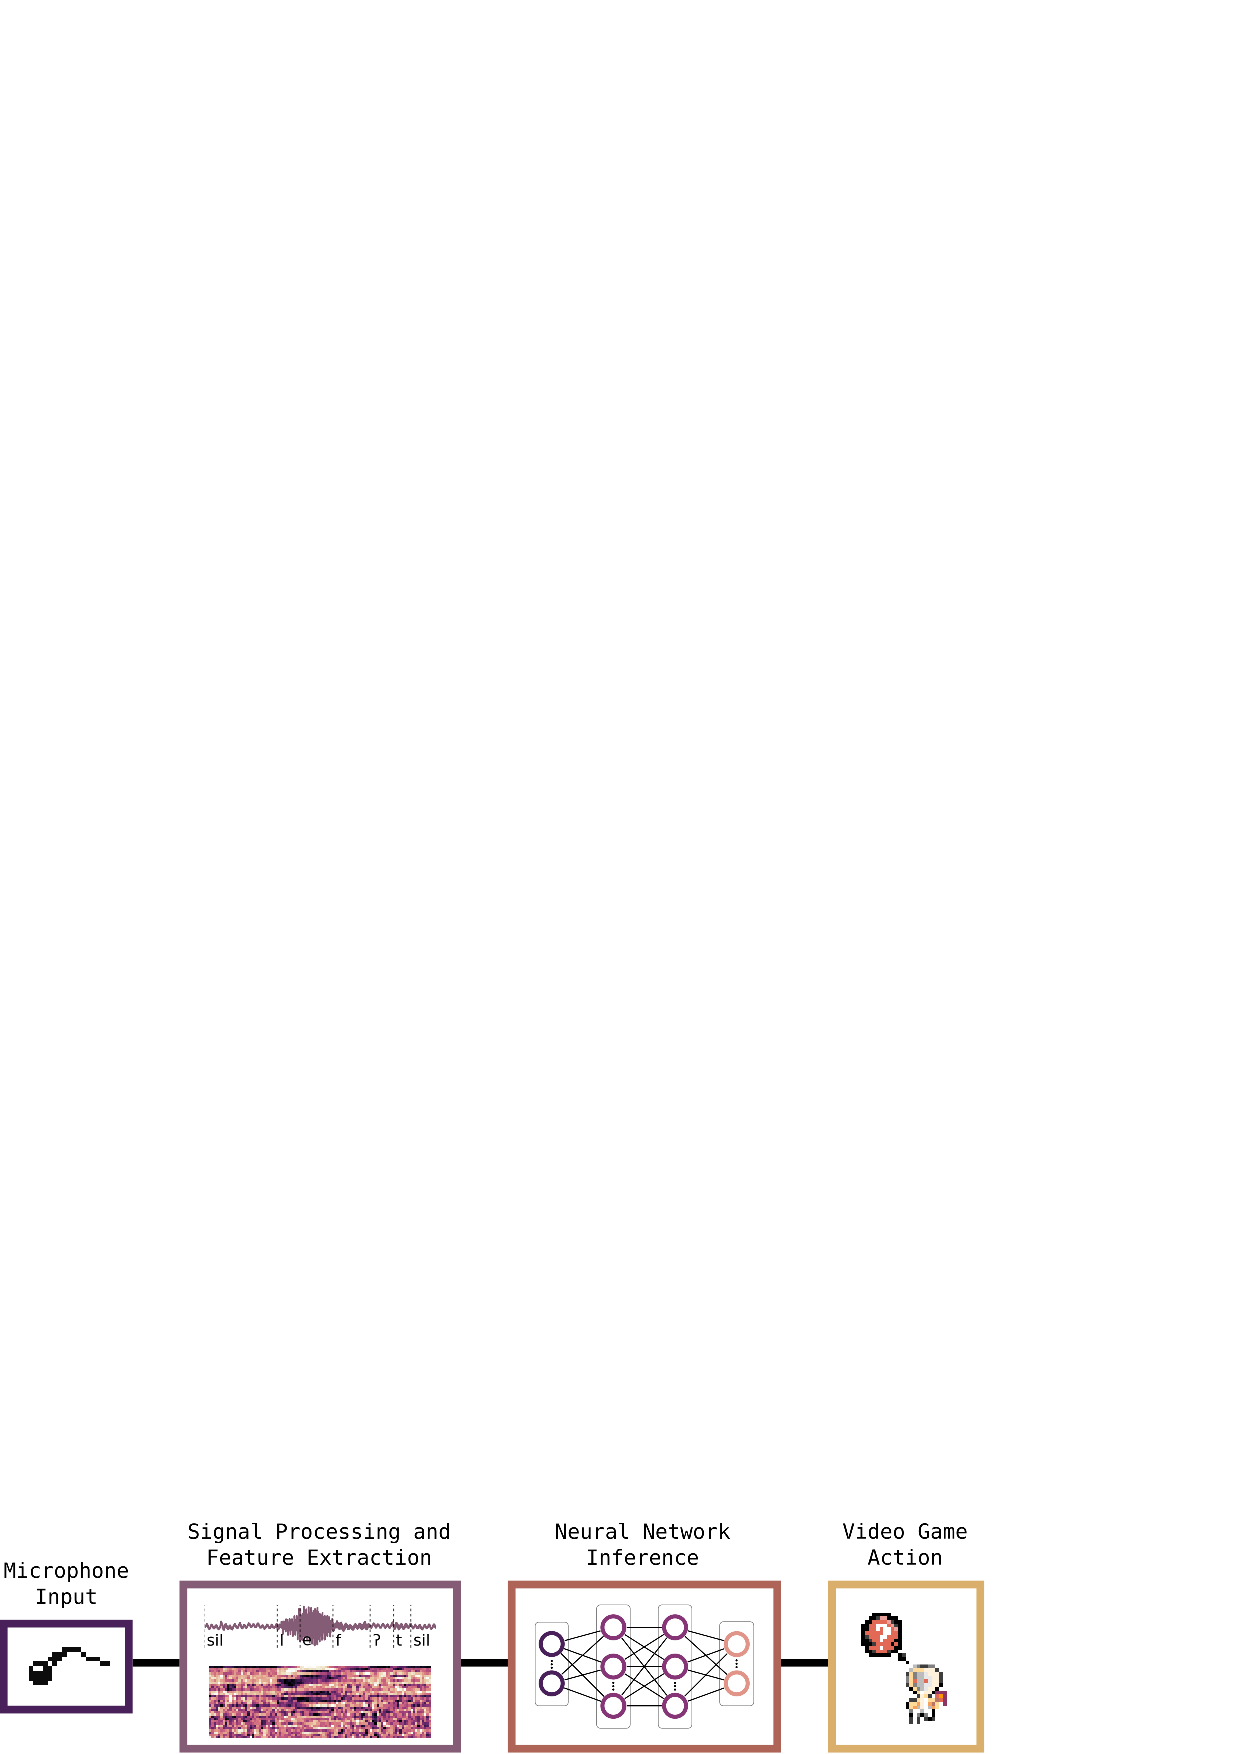
\includegraphics[width=0.95\textwidth]{./1_intro/figs/intro_kws.pdf}
  \caption{Simplified process of key word spotting for video games.}
  \label{fig:intro_kws}
\end{figure}
\FloatBarrier
\noindent
In the semantic perspective, the controlling of game objects, should be short, clear and best done with single command words, referred as speech commands.
Single words are easier to detect in comparison to long sentences, for instance, it is easier to recognize the word \enquote{left} than the sentence \enquote{missile target on position x, y}.
The classification of those speech commands can be done with a KWS system composed of a neural network.
KWS is restricted by a limited set of selected key words, referred as vocabulary or class dictionary.
In terms of video games, the set of key words might have members like \enquote{left} or \enquote{right}, for example, to move an element within the game to either left or right respectively.
The limited set of key words is crucial to restrict the complexity of the recognition task, since in practical applications it is not necessary to cover all words in a natural language.
Especially in video games, where the game environment is restricted by rules, technical limits and play-ability, KWS is suited perfectly as an alternative or augmented control system.
The size of the vocabulary and the selected words are two parameters that influence on one hand the choice of the neural network architecture, evaluated on energy efficiency and accuracy performance and on the other hand the game experience over the controls a player can choose from.
If the vocabulary of a KWS system would be too large, the chance of confusion between two different key words grows naturally.
In many KWS applications it is absolutely necessary to include labels for \emph{background noise}, \emph{silence} and \emph{unknown words} in the vocabulary. 
This is especially interesting in \emph{wake word} applications, where a single key word must be detected over the previously mentioned labels representing all other possible words that can be spoken.
Also in video games those additional labels are useful to prevent the player from eliciting unintended commands accidentally through, for instance, loud background noise.
Therefore, a KWS system has the demand of being very accurate and fast in its classification of key words.

Nowadays KWS systems are considered no science-fiction anymore, assisting consumers in everyday situations, such as rendering simple control tasks as the triggering of a photo release button on a \emph{smartphone} with a single speech command.
Application like this create more awareness of KWS, or generally speaking of speech recognition tasks, in human society.
Unfortunately some consumer applications with integrated speech recognition systems, leave a bitter aftertaste in data privacy issues and energy consumption through an externally and extensive computational processing pipeline over corporate servers \cite{Tang2018}.
It is therefore important to create incorporated KWS systems that respect private user data and provide an efficient implementation to save energy consumption.

Video games are a potential application for KWS, until now however, there exist very few of them taking advantage of this special feature.
Reasons for that might be found in the history of video games itself, where players find themselves in fast paced arcade games and speech recognition was simply too slow.
Additionally the complexity of KWS and lack of training data are often two valid arguments for not considering the deployment of a KWS system in a video game.

The following two sections in this introduction will briefly show the contributions of this thesis and give an overview of upcoming sections.
In summary, the focus of this thesis lies on KWS with neural networks trained through supervised learning on a speech command dataset \cite{Warden2018}.
The best suitable solutions for speech commands classification in video games are presented and evaluated with special interests in Convolutional Neural Networks (CNN), Generative Adversarial Neural Networks (GAN), and Wavenets.

% contributions
% --
% contributions

\section{Contributions}
The most of the effort is put into evaluating Convolutional Neural Network (CNN) models with low computational footprints, such as in \cite{Sainath2015}.
Besides low computational footprint, the depth of layers is hold to a minimum, so that it is still possible to get information about feature maps from the trained CNN networks.
The dataset used for the Key Word Spotting (KWS) task of those networks, was the speech command dataset \cite{Warden2018}.
The input features of the CNN models are the Mel Frequency Cepstral Coefficients (MFCC).
The amount of MFCC cepstral coefficients was evaluated with either 12 or 32 cepstral coefficients and showed that no accuracy improvements are achieved with 32 cepstral coefficients compared to 12.
The enhancement of MFCC to 39-feature vectors with 12 cepstral coefficients was also evaluated and showed only small improvements of accuracies, but not significant ones.
A frame-based normalization was performed on MFCCs to suite them better for visualization and use them for Generative Adversarial Networks (GAN) training.
Evaluation of the frame-based normalization was done in terms of accuracy, shift and noise invariance on conventional CNN models.
Frame-based normalization showed significant worse accuracies (about 5 to 10\%), it takes a bit longer for training, but improved in many experiments the noise invariance properties than without.
From those experiments the 12 cepstral coefficients with frame-based normalization were picked for further experiments.

Another large evaluation topic was that of GANs. 
With frame-based normalization the Generator (G) network was able to create convincing fakes to fool the Discriminator (D) network.
However it was found, when G and D are trained for too long, an equilibrium state where both generate random guesses or fakes might happen and the result is noise samples from G and a discrimination of D with slight changes around $0.5$.
Therefore a second loss term for G was added to create samples that have some similarity measure to the input data.
This helped to create better fakes and did not lead into noisy equilibrium states.

From the adversarial training of GAN networks, it was evaluated how their obtained weights through training can contribute in CNN models for KWS of speech commands.
Transfer learning was used to, transfer the obtained weights from either D or G to the equivalent CNN model.
With this approach it was possible to significantly increase the accuracy performance with about $3\%$ with using weights from G.
It showed that the obtained weights of G from an adversarial training can be very valuable.

A completely different approach for KWS was the evaluation of a Wavenet \cite{Oord2016} model for classification.
However with the hope that without feature extraction, a low computational model can be used, turned out to be extremely false.
Wavenets need a huge amount of operations by processing each sample from the audio files of the dataset.
Further the performances turned out to be very bad.
Nevertheless this model is evaluated and results are provided in hope for future research.

% overview
% --
% intro overview of thesis

\section{Overview of this thesis and notations}\label{sec:intro_overview}
\thesisStateReady
%This thesis is organized such, that each chapter leads to the next one and guiding someone who is interested in creating her own KWS game to follow through the process and challenges that might appear.
This thesis is organized that each chapter connects to the next one in a typical processing stage to create a KWS game.
% prev
After this introduction, \rsec{prev} provides information about previous and related work.
A small history sections about neural networks is given and important works on neural network architecture regarding this thesis are referrenced.
Further some works are presented that influenced and motivated this thesis.
Others works provide benchmarks on the used speech commands dataset or describe neural networks models that perform well on speech.
%In any way it is important to know, what is happening in the field of KWS and in which direction research is heading towards.
%Some works are used as motivation and some to get an idea.
% signal
\rsec{signal} is about audio signals processing and the extraction of meaningful features, such as MFCCs.
The feature extraction is explained in detail and examples are shown to visualize the results.
% neural networks
The used neural network architectures are described in \rsec{nn}. 
Further some theory of neural networks in general, CNNs, GANs and Wavenets is provided and highlighted with training results from experiments.
% experiments
In the \rsec{exp} information about the dataset and feature extraction is given and the experiments are presented.
Experiments are done on feature selection to determine the best suitable feature constellation the further experiments.
Adversarial pre-training is evaluated and Wavenets are compared to results from CNN based architectures.
% game
\rsec{game} describes the online and classification scheme in a possibile video game application.
Further some game design is presented and everything that is important for a KWS video game.
% conclusion
The thesis finishes with the conclusion in \rsec{conclusion}.


% visual guidance
%\subsection{Visual Guidance}\label{sec:intro_overview_visual}
%To get a better overview on the presentation of data and results, context specific color color-schemes are used within this thesis.
% There exist following context abstractions:

% \begin{itemize}
%     \item raw waveforms from soundfiles
%     \item extracted features, e.g. MFCCs
%     \item weights matrices of neural network models
%     \item training scores
% \end{itemize}

% ipa
\subsection{International Phonetic Alphabet}\label{sec:intro_overview_ipa}
The International Phonetic Alphabet (IPA) defines phonetics by human speaking sounds, where each symbol represents one specific sound.
A word formed with letters from a language alphabet, does not necessaryily represent the pronunciation of that word, therefore many dictionaries provide an IPA transcription so that no misconceptions may happen.
The plots, in some sections within this thesis, contain phonetic transcriptions with IPA characters, some of the more special ones are described in \rtab{intro_overview_ipa}.

% ipa table
\begin{table}[ht!]
\begin{center}
\caption{Some IPA and silence symbol with description.}
\begin{tabular}{ M{2cm}  M{9cm} }
\toprule
\textbf{IPA Symbol} & \textbf{Meaning} \\
\midrule
\textturnv & back vowel: \enquote{A}, open-mid roundend mouth \\
\textupsilon & back vowel: between \enquote{O} and \enquote{U}, nearly closed rounded mouth\\
\textinvglotstop & glottal stop\\
\midrule
sil & silence, no ipa symbol!\\
\bottomrule
\label{tab:intro_overview_ipa}
\end{tabular}
\end{center}
\end{table}
\FloatBarrier
\noindent



% math
\subsection{Mathematical Notations}\label{sec:intro_overview_math}
The mathematical equations or expressions are following some criteria.
Vectors and scalars are usually written in small letters with no special indication for vectors and matrices are written in capital letters.
The dimension of vectors and matrices are usually provided, such as $x\in\R^n$ or $X\in\C^{m \times n}$, or follow from the context.
Many letters like $n$ or $x$ are likewise used in different sections, but with different meaning and representations and should hopefully not confuse the reader of this thesis.
The letters $m$ and $n$ usually describes the length of a signal, $x$  and $y$ often represents input and output variables, etc.


% --
% background section

\chapter{Background}\label{sec:back}
This section provides fundamental background information regarding KWS, neural networks and video games.
The KWS task is described mathematically to express the actual speech recognition problem.
Notes on neural networks explain common properties and terms in their application.
Research questions are listed and give a deeper insight in common challenges of implementing a KWS system into a video game.

% disciplines
% --
% Intro of key word spotting

\section{The Key Word Spotting Task}\label{sec:intro_kws}
\thesisStateRevised
As described in \rsec{intro}, KWS is the task of classifying speech signals of spoken words to single key words out of a set of key words.
The set of key words $S$, also called vocabulary, can be defined as:
% kws dict
\begin{equation}\label{eq:intro_kws_dict}
	S \coloneqq \{s_i \mid i = 0, 1, \dots, L\}
\end{equation}
with a total number of $L$ key words denoted individually as $s_i$ for each key word.
The task is to select the key word closest to the spoken word from the user, denoted as target $t$.
The target does not necessarily have to be a member in the set of key words $S$, in fact it can be any arbitrary word.
With the abstract formulation:
% kws task
\begin{equation}\label{eq:intro_kws_task}
	\hat{s} = \underset{s_i \in S}{\arg \min} \, \mathcal{D}(t, s_i)
\end{equation}
the most probable key word $\hat{s}$ can be predicted, where $\mathcal{D}$ is some kind of distance measure between two words.
The formulation in \req{intro_kws_task} is merely semantic, but KWS in computer systems must cope with various transformations of raw input samples of audio data denoted as $\bm{x} \in \R^n$, with a total number of $n$ samples.
From the audio data an inference to output class probabilities $\bm{y} \in \R^L$ with a total number of $L$ class labels or key words, can be processed for instance with a neural network containing a softmax function at its last layer (transforming the output of the last layer to probability values).
With the softmax output from a neural network, the most probable key word can be picked by:
\begin{equation}\label{eq:intro_kws_class}
	\hat{s} = \{s_i \mid \underset{i = 0, 1, \dots, L}{\arg \max} \, y_i\}
\end{equation}
if the highest value of $y_i$ for all $i$ refers to the most probable index or indices of a spotted key word or key words in the vocabulary.

In comparison to full Automatic Speech Recognition (ASR), where whole sentences need to be identified, key word spotting operates merely on the word level.
Therefore KWS is a bit easier to deploy and less complex than ASR.
On the other hand KWS systems, that are used in practical applications, must run very energy efficiently on low energy devices, such as mobile phones, and give immediate and accurate responses to the users. 
A good elaboration on the requirements of KWS systems can be found in the motivation section of \cite{Warden2018}.
% --
% Intro to neural networks

\section{Neural Networks for Key Word Spotting}\label{sec:intro_nn}
\thesisStateReady
Neural networks enable computers to automatically learn from data to be able to solve tasks such as pattern recognition in images or audio.
The examples or samples from the input data can be paired with annotations, denoted as \emph{labels} or \emph{classes}.
If the label information of each example is used during the \emph{training} of a machine learning system, such as a neural network, it is called \emph{supervised learning} otherwise it is called \emph{unsupervised learning}, however supervised learning is more commonly applied.

%The big advantage of neural networks is that they are able to cope with huge amounts of input variables per data example and are able to extract their own features of those inputs through many layers within the network.
The big advantage of neural networks is that they are able to cope with large amounts of input variables per data example.
Considering a raw waveform file of merely \SI{1}{s} time duration, sampled with \SI{16}{\kilo\hertz} would give a input size of 16000 features.
This huge amount of input features is even difficult for neural networks to learn from and usually a feature extraction stage is placed in between to reduce the input dimension.
For instance the computation of MFCCs, using 12 out of 32 coefficients and a time duration of \SI{0.5}{s} with a time shift of \SI{10}{\milli\second}, reduces the input feature size dramatically to $12 \times 50 = 600$, which is still a high number of input features, but much more affordable and faster to train.

%In this thesis, the word \emph{feature} has several meanings, one is as name of extracted data and therefore be the same as input variables. 
%Another is, that a feature is simply some kind of compressed representation of a high dimensional data.
Neural networks are able to learn own feature representations, selection and interpretation, rather than using hand-crafted ones done by humans with expertise in the application.
Note that hand-crafting features of a complex recognition task, is in most cases not even possible or extremely cumbersome.
So researchers prefer neural networks because of their easy deployment scheme and state of the art performances.
Further it enables everyone who is capable of using neural network tools, to create solution to rather complex problems usually solved by experts in the field, given there is enough data and processing power available.
Therefore elaborate feature extraction stages become less important to the users.
This on the other side may lead into less understanding of the actual problem and more \enquote{try and error} approaches of different neural network architectures and training parameters.
The energy consumption required to train large neural network with many parameters on a huge training dataset, shall not be forgotten, especially in times of climatic change.
Reusing pre-trained weights from renowned network architectures is a good way to reduce energy consumption in finding an optimal classifier for a specific task.
The re-usability of pre-trained weights is often named as \emph{transfer learning}. 
A small summary on transfer learning can be found in \cite{TransferLearning}.
%This led to the thinking that everyone, who owns data and computational power, is the superior of solving complex problems such as image or audio classifications.
%However it is not always like this rather negative example, when using neural network approaches.

The potential of neural networks in research are vast.
The observation on how the learning from data is done and what recognition patterns are obtained after training, might allow researchers and experts to better understand the problem or gain a different viewpoint on it.
%However if neural networks are observed on how they are able to learn from data and what recognition patterns they have obtained after training, it might benefit researchers and experts to better understand the problem or gain a different viewpoint on it.
%It is extremely interesting to work with them and get knowlege about how and why they are able to produce such good results.
%This again feedbacks experts to gain more understanding or a different viewpoint on the topic.
Especially when using Convolutional Neural Networks (CNN), researchers are actually able to observe and visualize the learned filters and interpret the results.
A very interesting example of investigating learned CNN filters is shown by Zeiler el. al. \cite{Zeiler2013}.
Other interesting subjects in research are generative models, such as Generative Adversarial Networks (GAN) \cite{Goodfellow2014}, which are able to create convincing samples from the learned data distribution.

Neural network architectures for speech recognition are a little bit different from image recognition, mainly because of the sequential nature of time signals.
However if time signals are restricted in time, that means limited to a fixed number of samples, and frequency features are extracted over that time span, then speech signals can be represented in 2D space (frequency and time) and classified like images.
That suggests that CNNs are reasonable network architectures for speech as well.
Another interesting architecture for audio signals is the Wavenet \cite{Oord2016}, because of its ability to process raw audio data.
%and were originally intended for speech synthesis, but could also be used for recognition tasks.



% --
% video games with speech commands

\section{Video Games with Speech Input}\label{sec:intro_games}
\thesisStateReady
Video games with speech inputs are a rarely seen occurrence in the gaming industry, though it is a very interesting and immersive way to interact.
Technically the voice of the player of the video game, has to be recorded by a microphone, therefore one additional requirement of being able to play the video game is to own a microphone, which however does not need to be high-end.
The input stream of a microphone can be processed through an online or realtime system to extract the input data for the classification system.
The classification system, such as a neural network, infers the input data and therefore hopefully the intention of the player to a real action within the game.
The processing scheme is easy to define, but not that easy to implement compared to other more hardware based input channels, such as a click on a keyboard button.
Also speech input is very slow compared to hardware input, where players interact within tens of milliseconds (the input lag of gaming controllers should ideally be under \SI{50}{\milli\second}).
This is not possible with speech, the player has to physically form a waveform representing the action in the game.
Further the waveform captured from the online system has to be pre-processed, feature extracted and classified to the best estimation of all the available key words in the games vocabulary.
Concluding this, a good estimate to create and process a speech input should ideally be under one second, the less the better for the playing experience.

Another important question is how many key words or speech commands, should be used for the vocabulary.
A high number of key words will increase the chance of confusion and a small number of key words restrict the possible actions a player can choose from.
The possibility to create separate classifiers with different sets of smaller vocabularies of speech commands arises depending on which commands the player actually needs in the actual scenario within the video game. For instance if the player is in a dialogue with a Non Player Character (NPC) it makes sense to reduce the vocabulary to only \{\enquote{yes}, \enquote{no}\} if those are the only actions to choose from.

The use of labels for background noise, silence and unknown words depends on the game and how the classification process is activated.
If the assumption is made that a player chooses only from the key words in the dictionary, then the label of unknown words is not really necessary.
However the unknown label would be very interesting if key words are not that common to a player, such as words from a different language or fantasy words.
The unknown label will therefore motivate the player to correctly pronounce the word itself, which could be also used in language learning games.
The labels for background noise and silence are useful if the activation of the classification process is initiated by the energy value of the input stream of the microphone.
A stroke on the microphone or loud background sound can therefore elicit an unwanted command within the game, if those labels do not exist.

In any case there are much problems to consider when using KWS in video games and probably therefore hinders game developers to produce more content with it.

%Maybe those issues and the complexity of the task hinders game developers to produce more content with Key Word Spotting.
% A speech input for video games is a spoken waveform, recorded through a microphone, from any speaker intending to inflict a certain change while playing a Video Game. 
% Certainly this spoken waveform has to be processed, such as other inputs channels have to be (like keyboard buttons pressed), so that its meaning can be understood by the computer system behind the game. 
% Although this processing of a waveform is much more complicated and prone to errors, compared to a simple click on the keyboard or mouse. 
% That might be one of the reasons why Speech Inputs are very rare to be found in Video Games, still they exist.

% research questions
% --
% research questions

\section{Research Questions for this Thesis}\label{sec:intro_rq}
This section formulates relevant research questions regarding KWS in video games.
Those research questions can be split into 3 parts:
\begin{enumerate}[label={Q.\arabic*)}, leftmargin=1.4cm]
  \item Signal processing and feature extraction of speech signals.
  \item Neural network training and classification for KWS.
  \item Video games with KWS.
\end{enumerate}
Note that the terms \enquote{key word} and \enquote{speech command} are often named interchangeably because speech commands are used as key words in the KWS system.
Not all research questions can be answered within the scope of this thesis.
Nevertheless, those questions can be asked and some solution concepts discussed.


% --
% signal

\subsection{Signal Processing and Feature Extraction Research Questions}\label{sec:intro_rq_signal}
Acquiring meaningful features from speech signals is essential for neural networks to operate on. 
The features are extracted from raw audio samples of a microphone input stream in a specific time interval.
Those retrieved features are further input to a neural network for the classification of speech commands.
The following Questions arise here:
\begin{enumerate}[label={Q.1.\alph*)}, leftmargin=1.75cm]
  \item Which time interval should be captured to represent a speech command?\label{it:q1-a}
  \item Does the signal processing have to be invariant to background noise and especially to game sounds?\label{it:q1-b}
  \item What are meaningful features for speech recognition?\label{it:q1-c}
\end{enumerate}
\noindent
\textbf{Question \ref{it:q1-a}:} 
The time required to fully pronounce a speech command is not fixed and varies from speaker to speaker, depending also on the intended prolongation a speaker adds to the word.
In practical applications however, a fixed time interval for a single speech command is convenient.
By restricting the time duration of the key words, the speaker has to pronounce the words within this time span.
For example, if a speaker pronounces the word \enquote{left} and requires a time duration of \SI{1}{\second}, hardly all is captured if the time interval is restricted to merely \SI{500}{\milli\second}.
Whether this \SI{500}{\milli\second} is sufficient for a correct classification, is subject for evaluation.
In the application of a video game, the user should preferably speak the commands with a short time duration so that the game can respond fast.
Problems might occur if the speech commands are spoken repeatedly and very hasty such that the time interval of consecutive commands overlap each other.
Ideally the time interval to represent a speech command would be flexible but this more difficult to implement than a fixed time interval.

\textbf{Question \ref{it:q1-b}:}
Usually the presence of low background noise should not be a problem for neural networks trained on a large enough data set. 
The game sounds might present a more difficult problem, when turned up too loud without the use of headphones. 
Therefore, the microphone will not only capture the voice of a speaker but also a fair amount of game sounds. 
This problem seems to be theoretically solvable as the shape of the nuisance is known and the amount of game sound in the audio stream could be attenuated sufficiently.
In practice this might be hard to solve without critically disturbing the signal of interest.
A solution to this problem would probably take too much time and effort and is therefore not evaluated within this thesis. 
However, playing a video game without game sound is unsatisfying and it would be a great contribution to tackle this problem in future work.

\textbf{Question \ref{it:q1-c}:} 
The determination of meaningful features for speech signals is a classical problem in speech recognition.
The essential composition of a word may help to understand the problematic better.
A word is a sequential combination of either vowels, such as \enquote{a} and \enquote{e}, or consonants \enquote{k}, \enquote{l}, with a certain length. 
In linguistics, for instance, it is possible to distinguish vowels with frequency peaks in a spectrogram, where a spectrogram is the magnitude squared of the frequency response of small time chunks over the time duration of a signal.
However, due to many different factors in voice generation involved in speakers, such as age, gender, nationality and physiology of the vocal tract, there is a huge variance in the pronunciation of words from different persons, which increases the difficulty of the problem.
A very common approach is to use MFCCs as features for speech recognition tasks.
Why MFCCs present reasonable features for speech, is described in detail in \rsec{signal_mfcc}.


% --
% neural networks

\subsection{Neural Network Implementation Research Questions}\label{sec:intro_rq_nn}
Neural networks for video games should ideally be very efficient and provide accurate classifications of input features.
The vocabulary in a KWS task has to be specified for the individual game and chosen from all class labels available in the dataset.
Each key word of the vocabulary is presented by one output node of the neural network architecture.
Following Questions can be asked in general:
\begin{enumerate}[label={Q.2.\alph*)}, leftmargin=1.75cm]
  \item Is there an appropriate dataset suited for KWS video games and with sufficient diversity available?\label{it:q2-a}
  \item What happens if an input feature represents a spoken word, which is not in the vocabulary (unknown key word) and how should this exception be handled?\label{it:q2-b}
  \item What is the best neural network architecture regarding classification accuracy and energy efficiency?\label{it:q2-c}
  \begin{enumerate}[label=(\roman*)]
    \item Can adversarial networks improve generalization?
    \item Are Wavenets a solution to this task?
  \end{enumerate}
\end{enumerate}
\noindent
\textbf{Question \ref{it:q2-a}:} 
The availability of a dataset for KWS video games can be answered right away, as there exists a speech commands dataset \cite{Warden2018} with enough and diverse data.
The dataset consist of 35 labels and contains commands for movement and numbers.
Further, it includes randomly selected words like \enquote{marvin} or \enquote{bird} intended to represent \emph{unknown} words for the KWS system.
It has to be noted that not every game idea can be realized with a restricted vocabulary.
Nevertheless, with commands for movement like \enquote{left} or \enquote{go} it is possible to move objects within a game and this can already be used for many game mechanics.
An aspect regarding efficiency, is to restrict the amount of key words in the vocabulary as much as possible such that a cheaper neural network architecture can be deployed, which of course should still be sufficiently good in its classification accuracy.

\textbf{Question \ref{it:q2-b}:} 
Without doubt, players will try out words that are not in the vocabulary (denoted as \emph{unknown} key words) and observe the response of the video game.
The ideal response would be to shown an indication to the player that the word is not present in the vocabulary. 
Nevertheless, it might happen that the similarity of an unknown key word is too close to a key word and an unintended action is triggered in the game. 
At the same time the neural network should not classify key words as unknown key words to ensure a satisfying game experience.
It is better to rely on that players are using key words for most of the time so that they are preferred over unknown key words.

\textbf{Question \ref{it:q2-c}:}
In the ideal case, video games with KWS do not slow down during the inference process of unknown input data.
The restriction of the amount of computations and time for the classification of key words is given by the minimum Frames Per Second (FPS) a video game is perceived as fluent.
That requires the FPS to not fall under a certain limit (usually 30 FPS in video games), otherwise the fluidity of the game is not guaranteed.
Therefore, several different neural network approaches with a low computational footprint have to be tested and compared against each other regarding classification rate and energy efficiency.
The transfer of weights from GANs is an interesting approach to evaluate whether the trained parameters are also useful for pure classification tasks in CNNs.
Wavenets have the advantage that they do not need a feature extraction stage but it is questionable whether the network design achieves a reasonable computational footprint.


% --
% video games

\subsection{Video Games with KWS Research Questions}\label{sec:intro_rq_games}
Video games that use KWS can create an unique playing experience but have to face certain challenges.
Following questions can be stated:
\begin{enumerate}[label={Q.3.\alph*)}, leftmargin=1.75cm]
  \item How should the onset of a key word be detected, so to reduce computations?\label{it:q3-a}
  \item What is the added value of KWS in the gaming experience of players?\label{it:q3-b}
  \item What do game developers have to consider, when designing a game with KWS?\label{it:q3-c}
\end{enumerate}
\noindent
\textbf{Question \ref{it:q3-a}:} 
It is crucial to reduce computations in a video game in order to keep it running fluently during high performance peaks.
Also the unnecessary processing of meaningless input data should be avoided as much as possible.
Ideally the key word classification is activated, when there is actually a speech command present, which however is not always trivial.
One possibility to indicate the onset of a key word is to perform the relatively efficient calculation of an energy value within a certain time interval of the raw input data stream and have a simple threshold value decide, whether a speech command is available. 
To avoid the consecutive triggering of onsets at each energy measure, the microphone and amplifier noise floor and the background sound (including the game sound) have to be less energy intensive than the speech signal obtained from the player.
Another approach similar to the push and talk principle, would be to indicate the onset of a key word with the click of a certain button on the keyboard.
The player is therefore able to control the exact onset of a key word and its length but requires an additional hardware based input channel.

\textbf{Question \ref{it:q3-b}:}
In certain video game scenarios, speech commands can be useful, interesting and enhancing for the gaming experience, in others they might even disturb the game play or even spoil it completely.
It cannot be generally stated whether it is worth to deploy a KWS system into a game, this depends on the game it is intended for.
As already noted in \rsec{intro_games}, KWS might be a great augmented control system for special kind of games to increase the immersion experience, especially for VR applications.
Also language learning games are an interesting application but usually require a huge vocabulary and therefore a phoneme based ASR system would be the better choice.

\textbf{Question \ref{it:q3-c}:}
Apart from the technical requirements involved in KWS systems, also the general game design with KWS has to be considered.
It certainly can be stated that KWS systems are not always reliable and therefore a main game mechanic solely based on it is not always preferred.
Furthermore, the time lag required to process speech commands to actual actions within the game should not be ignored.
The player should get on the one hand immediate and accurate feedback from the game and on the other hand be challenged while playing.
Further, by achieving both criteria it ensures that the game experience does not suffer from getting frustrating or tiresome.
Additionally it must be considered, that players might get exhausted by using speech commands consecutively in short intervals during the game.
Therefore, the players might prefer a game design where they have to use KWS only in special situations.
As general conclusion, it can be stated that a game developer has to design a KWS game with great care.